\documentclass[10pt,aspectratio=169]{beamer}

\usetheme{default}
\usecolortheme{default}
\usefonttheme{professionalfonts}

\usepackage[T1]{fontenc}
\usepackage{lmodern}
\usepackage{booktabs}
\usepackage{array}
\usepackage{tabularx}
\usepackage{tikz}
\usetikzlibrary{arrows.meta,positioning,calc,fit,decorations.pathreplacing}

% ---------------------------
% Easy-to-replace placeholders
% ---------------------------
\newcommand{\TrainPeriod}{through 2022-12-31}
\newcommand{\DiscoveryPeriod}{2023-01-01 to 2023-12-31}
\newcommand{\ValidationPeriod}{2024-01-01 to 2024-12-31}
\newcommand{\TestPeriod}{after 2024-12-31}

\newcommand{\MaxIterations}{5}

\newcommand{\IterOneChange}{[INITIAL HYPOTHESIS]}
\newcommand{\IterTwoChange}{[REVISION]}
\newcommand{\IterThreeChange}{[REVISION]}
\newcommand{\IterFourChange}{[REVISION]}
\newcommand{\IterFiveChange}{[REVISION]}

\newcommand{\IterOneRankIC}{[IC1]}
\newcommand{\IterTwoRankIC}{[IC2]}
\newcommand{\IterThreeRankIC}{[IC3]}
\newcommand{\IterFourRankIC}{[IC4]}
\newcommand{\IterFiveRankIC}{[IC5]}

\newcommand{\IterOneSharpe}{[S1]}
\newcommand{\IterTwoSharpe}{[S2]}
\newcommand{\IterThreeSharpe}{[S3]}
\newcommand{\IterFourSharpe}{[S4]}
\newcommand{\IterFiveSharpe}{[S5]}

\newcommand{\IterOneTurnover}{[T1]}
\newcommand{\IterTwoTurnover}{[T2]}
\newcommand{\IterThreeTurnover}{[T3]}
\newcommand{\IterFourTurnover}{[T4]}
\newcommand{\IterFiveTurnover}{[T5]}

\newcommand{\DiscoveryRankIC}{[DISCOVERY RANK IC]}
\newcommand{\ValidationRankIC}{[VALIDATION RANK IC]}
\newcommand{\DiscoverySharpe}{[DISCOVERY SHARPE]}
\newcommand{\ValidationSharpe}{[VALIDATION SHARPE]}
\newcommand{\DiscoveryTurnover}{[DISCOVERY TURNOVER]}
\newcommand{\ValidationTurnover}{[VALIDATION TURNOVER]}
\newcommand{\DiscoveryPValue}{[DISCOVERY P]}
\newcommand{\ValidationPValue}{[VALIDATION P]}
\newcommand{\ValidationDecision}{[PASS / REJECT]}
\newcommand{\ExampleInterpretation}{[Describe how the Critic identified a weakness and how the Improver reacted.]}
\newcommand{\InitialThesis}{[INITIAL THESIS]}
\newcommand{\EmpiricalContradiction}{[EMPIRICAL CONTRADICTION]}
\newcommand{\CriticInterpretation}{[CRITIC INTERPRETATION]}
\newcommand{\RevisedThesis}{[REVISED THESIS]}

% ---------------------------
% Visual system
% ---------------------------
\definecolor{Ink}{HTML}{18202A}
\definecolor{Muted}{HTML}{59636F}
\definecolor{Accent}{HTML}{1F6F78}
\definecolor{AccentSoft}{HTML}{E5F1F2}
\definecolor{Rule}{HTML}{CBD5DD}
\definecolor{Warn}{HTML}{8A4B18}
\definecolor{WarnSoft}{HTML}{FFF2DD}
\definecolor{CodeBg}{HTML}{F4F7F9}

\setbeamercolor{normal text}{fg=Ink,bg=white}
\setbeamercolor{frametitle}{fg=Ink,bg=white}
\setbeamercolor{title}{fg=Ink,bg=white}
\setbeamercolor{subtitle}{fg=Muted,bg=white}
\setbeamercolor{structure}{fg=Accent}
\setbeamercolor{footline}{fg=Muted,bg=white}
\setbeamercolor{block title}{fg=Ink,bg=AccentSoft}
\setbeamercolor{block body}{fg=Ink,bg=AccentSoft}

\setbeamertemplate{navigation symbols}{}
\setbeamertemplate{itemize item}{\color{Accent}\small$\blacktriangleright$}
\setbeamertemplate{itemize subitem}{\color{Accent}\scriptsize$\bullet$}
\setbeamertemplate{frametitle}{%
  \vspace{0.35cm}
  \insertframetitle\par
  \vspace{0.12cm}
  {\color{Rule}\rule{\textwidth}{0.4pt}}
}
\setbeamertemplate{footline}{%
  \leavevmode%
  \hbox{%
    \begin{beamercolorbox}[wd=.72\paperwidth,ht=2.6ex,dp=1.0ex,leftskip=0.45cm]{footline}%
      Alec Hewitt
    \end{beamercolorbox}%
    \begin{beamercolorbox}[wd=.28\paperwidth,ht=2.6ex,dp=1.0ex,rightskip=0.45cm plus1fil]{footline}%
      \hfill\insertframenumber/\inserttotalframenumber
    \end{beamercolorbox}%
  }%
}

\setlength{\parindent}{0pt}
\setlength{\parskip}{4pt}
\renewcommand{\arraystretch}{1.15}

\newcommand{\code}[1]{\texttt{\small #1}}
\newcommand{\placeholder}[1]{\textcolor{Warn}{\textbf{#1}}}

\tikzset{
  box/.style={draw=Rule, rounded corners=2pt, fill=white, thick, align=center, inner sep=6pt, minimum height=0.78cm},
  llmbox/.style={box, draw=Accent, fill=AccentSoft},
  codebox/.style={box, draw=Ink!35, fill=CodeBg},
  arrow/.style={-{Latex[length=2.2mm]}, thick, draw=Accent},
  faintarrow/.style={-{Latex[length=2.0mm]}, thick, draw=Muted!70},
  gate/.style={draw=Accent, fill=AccentSoft, rounded corners=2pt, thick, align=center, inner sep=5pt}
}

\title{Designing an Agentic AI Alpha Researcher}
\subtitle{A bounded hypothesis-generation, evaluation, and refinement framework}
\author{}
\institute{Prototype research system}
\date{}

\begin{document}

% Slide 1
\begin{frame}[plain]
  \vspace{1.2cm}
  {\Large\bfseries Designing an Agentic AI Alpha Researcher}

  \vspace{0.25cm}
  {\normalsize\color{Muted} Alec Hewitt}

  \vfill
  {\color{Rule}\rule{\textwidth}{0.4pt}}
  {\small\color{Muted} Prototype research system \hfill }
\end{frame}

\begin{frame}{Presentation Overview}

    \tableofcontents

\end{frame}



\section{Task (Topic B) Overview}
% Slide 2
\begin{frame}{Task (Topic B)}
  \begin{block}{Objective}
    Build an agentic research system that can
    \textbf{propose, evaluate, critique, and revise}
    quantitative alpha hypotheses using empirical feedback.\\
   \textbf{Research Agent: Propose} $\rightarrow$ \textbf{Code: Evaluate} $\rightarrow$ \textbf{Critic Agent: Critique}\\
   $\rightarrow$ \textbf{Improver Agent: Revise}
  \end{block}
  \small
  \begin{columns}[T,onlytextwidth]
    \begin{column}{0.47\textwidth}
      \textbf{Inputs}
      \begin{itemize}
        \item Engineered market features (volatility\_20d, relative\_volume, etc.)
       \item Proposed signals evaluated against realized 5-day forward returns
       \item OpenAI API for agent reasoning (5.6-Luna)
      \end{itemize}
    \end{column}
    \begin{column}{0.47\textwidth}
      \textbf{Outputs}
      \begin{itemize}
        \item Economic thesis
        \item Executable alpha signal definition
        \item Quantitative evaluation metrics
        \item Agent iteration history
        \item Final validation / test decision
      \end{itemize}
    \end{column}
  \end{columns}

  \vspace{0.18cm}

 % \vspace{0.05cm}
  %{\footnotesize\textbf{Prototype data universe:} daily price/volume data feed lagged or rolling features computed at or before the prediction date: \code{momentum\_20d}, \code{momentum\_20d\_rank}, \code{momentum\_20d\_z}, \code{volatility\_20d}, \code{relative\_volume}, \code{vol\_rolling\_avg}.}
\end{frame}

\section{Input Data}

\begin{frame}{Data and Feature Construction}

\small

\begin{columns}[T]

% ---------------- LEFT ----------------
\begin{column}{0.46\textwidth}

\textbf{Raw daily market data}

\vspace{0.15cm}

\begin{tabular}{ll}
\toprule
Field & Meaning \\
\midrule
date   & trading date \\
ticker & stock identifier \\
close  & daily closing price \\
volume & daily trading volume \\
\bottomrule
\end{tabular}

\vspace{0.35cm}

One observation corresponds to a
\textbf{stock--date pair}.

\vspace{0.35cm}

\textbf{Prediction target}

\[
r^{(5)}_{i,t}
=
\frac{P_{i,t+5}}{P_{i,t}}-1
\]

{\scriptsize
Future 5-day return is used only as the evaluation target,
not as an input to the signal.
}

\end{column}

% ---------------- RIGHT ----------------
\begin{column}{0.50\textwidth}

\textbf{Engineered features available to the agent}

\vspace{0.12cm}

\[
\text{return}_{5d}
=
\frac{P_t}{P_{t-5}}-1
\]
{\scriptsize Short-term trailing price return}

\vspace{0.12cm}

\[
\text{momentum}_{20d}
=
\frac{P_t}{P_{t-20}}-1
\]
{\scriptsize Medium-term trailing price momentum}

\vspace{0.12cm}

\[
\text{volatility}_{20d}
=
\operatorname{Std}
(r_{t-19},\ldots,r_t)
\]
{\scriptsize Recent realized return volatility}

\vspace{0.12cm}

\[
\text{relative volume}
=
\frac{V_t}{\overline{V}_{20d}}
\]
{\scriptsize Current volume relative to recent average volume}

\vspace{0.15cm}

%{\footnotesize Together these provide the agent with information about \textbf{short-term returns, medium-term trend, risk, and trading activity}.}

\end{column}

\end{columns}

\vspace{0.2cm}

\begin{block}{No look-ahead in feature construction}
All signal features at date $t$ use only information available
at or before $t$.
\end{block}

\end{frame}
\section{Architecture Overview}
\begin{frame}{System Architecture}
  \small
\centering
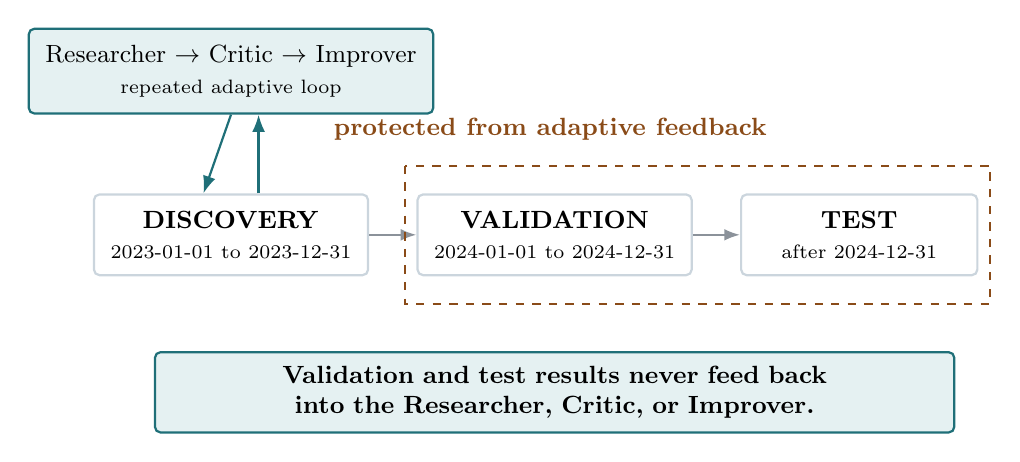
\begin{tikzpicture}[font=\small]

  % Data splits
  \node[box, minimum width=3.0cm, minimum height=1.0cm] 
  (disc) at (0,0) {
    \textbf{DISCOVERY}\\
    {\scriptsize \DiscoveryPeriod}
  };

  \node[box, minimum width=3.0cm, minimum height=1.0cm, right=0.6cm of disc] 
  (valid) {
    \textbf{VALIDATION}\\
    {\scriptsize \ValidationPeriod}
  };

  \node[box, minimum width=3.0cm, minimum height=1.0cm, right=0.6cm of valid] 
  (test) {
    \textbf{TEST}\\
    {\scriptsize \TestPeriod}
  };

  % Forward data flow
  \draw[faintarrow] (disc) -- (valid);
  \draw[faintarrow] (valid) -- (test);

  % Agentic research loop
  \node[
    llmbox,
    above=1.0cm of disc,
    minimum width=3.9cm
  ] 
  (loop) {
    Researcher $\rightarrow$ Critic $\rightarrow$ Improver\\
    {\scriptsize repeated adaptive loop}
  };

  \draw[arrow] (loop.south) -- ($(disc.north)+(-0.35,0)$);
  \draw[arrow] ($(disc.north)+(0.35,0)$) -- ($(loop.south)+(0.35,0)$);

  % Protected validation/test region
  \draw[
    draw=Warn,
    thick,
    dashed
  ] 
  ($(valid.north west)+(-0.15,0.35)$) 
  rectangle 
  ($(test.south east)+(0.15,-0.35)$);

  \node[
    align=center,
    color=Warn,
    above=0.55cm of valid
  ] 
  (firewall) {
    \textbf{protected from adaptive feedback}
  };

  % Design rule
  \node[
    gate,
    below=0.95cm of valid,
    text width=9.8cm
  ] {
    \textbf{Validation and test results never feed back into the Researcher, Critic, or Improver.}
  };

\end{tikzpicture}

\end{frame}


% Slide 3
\begin{frame}{Agentic Loop}
  \centering
\resizebox{\textwidth}{!}{%
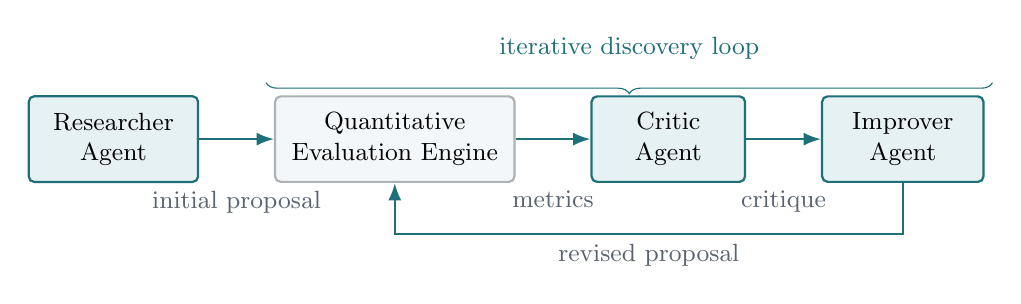
\begin{tikzpicture}[node distance=0.8cm and 0.95cm, font=\small]

  \node[llmbox, minimum width=2.15cm] 
    (researcher) {Researcher\\Agent};

  \node[codebox, right=of researcher, minimum width=2.65cm] 
    (engine) {Quantitative\\Evaluation Engine};

  \node[llmbox, right=of engine, minimum width=1.95cm] 
    (critic) {Critic\\Agent};

  \node[llmbox, right=of critic, minimum width=2.05cm] 
    (improver) {Improver\\Agent};

  % Initial proposal
  \draw[arrow] (researcher) -- 
    node[below, yshift=-15pt, color=Muted] {initial proposal} 
    (engine);

  % Evaluation feedback
  \draw[arrow] (engine) -- 
    node[below, yshift=-15pt, color=Muted] {metrics} 
    (critic);

  % Critique
  \draw[arrow] (critic) -- 
    node[below, yshift=-15pt, color=Muted] {critique} 
    (improver);

  % Revised proposal feeds directly back to evaluator
  \draw[arrow] (improver.south) -- ++(0,-0.65) -|
    node[pos=0.25,below,color=Muted] {revised proposal}
    (engine.south);

  \draw[
    decorate,
    decoration={brace,mirror,amplitude=4pt},
    draw=Accent
  ]
  ($(engine.north west)+(-0.1,0.16)$) --
  ($(improver.north east)+(0.1,0.16)$)
  node[midway,above=5pt,color=Accent]
  {iterative discovery loop};

\end{tikzpicture}
}


\end{frame}

\section{Researcher Agent}
\begin{frame}{Researcher Agent: Generate the Initial Hypothesis}

\small

\begin{block}{Purpose}

The Researcher Agent generates the \textbf{initial alpha proposal} that seeds the iterative research loop.

\end{block}

\vspace{0.15cm}

\begin{columns}[T,onlytextwidth]

% ---------------- LEFT ----------------
\begin{column}{0.47\textwidth}

\textbf{Information provided}

\begin{itemize}
    \item Available engineered features:
    \begin{itemize}
        \item \code{return\_5d}
        \item \code{momentum\_20d}
        \item \code{volatility\_20d}
        \item \code{relative\_volume}
    \end{itemize}

    \item Allowed operations:
    \[
    +,\quad -,\quad \times,\quad \div
    \]
\end{itemize}

\end{column}

% ---------------- RIGHT ----------------
\begin{column}{0.49\textwidth}

\textbf{Output: initial proposal}

\vspace{0.1cm}

The Researcher must return:

\begin{itemize}
    \item two features: $x_1,x_2$
    \item operation $f$
    \item weights $w_1,w_2$
    \item economic thesis
\end{itemize}

\vspace{0.1cm}

\[
\alpha_{i,t}
=
f\!\left(
w_1 x_{1,i,t},
w_2 x_{2,i,t}
\right)
\]

\vspace{0.15cm}

\end{column}

\end{columns}

\vspace{0.15cm}


\end{frame}

\section{Evaluation Engine}
\begin{frame}{Quantitative Evaluation Engine: Test the Proposal}

\small

\begin{block}{Purpose}
The Quantitative Evaluation Engine \textbf{deterministically backtests}
each proposed alpha signal against historical forward returns.
\end{block}

\vspace{0.15cm}

\begin{columns}[T,onlytextwidth]

% ---------------- LEFT ----------------
\begin{column}{0.47\textwidth}

\textbf{Information provided}

\begin{itemize}
    \item Alpha proposal: \[\alpha_{i,t} = f\!\left( w_1x_{1,i,t}, w_2x_{2,i,t} \right) \]

    \item Historical discovery data

    \item Realized 5-day forward returns
\end{itemize}

\vspace{0.15cm}

\end{column}

% ---------------- RIGHT ----------------
\begin{column}{0.49\textwidth}

\textbf{Output: metrics}

\vspace{0.1cm}

For each date, stocks are ranked by
$\alpha_{i,t}$ and compared with their
realized forward returns.

\vspace{0.15cm}

\begin{itemize}
    \item \textbf{Mean Rank IC}\\
    {\scriptsize Did the signal correctly rank future relative returns?}

    \item \textbf{Sharpe ratio}\\
    {\scriptsize Did the ranking produce consistent long--short returns?}

    \item \textbf{Mean turnover}\\
    {\scriptsize How much did portfolio positions change over time?}
\end{itemize}

\vspace{0.1cm}

\end{column}

\end{columns}

\end{frame}

\section{Critic Agent}
\begin{frame}{Critic Agent: Diagnose the Weakness}

\small

\begin{block}{Purpose}
The Critic Agent interprets the \textbf{metrics from the evaluation engine}
and identifies the main weakness of the current alpha proposal.
\end{block}

\vspace{0.15cm}

\begin{columns}[T,onlytextwidth]

% ---------------- LEFT ----------------
\begin{column}{0.47\textwidth}

\textbf{Information provided}

\begin{itemize}
    \item Current alpha proposal: 

    \begin{itemize}
   	\item $\alpha_{i,t} = f\!\left( w_1x_{1,i,t}, w_2x_{2,i,t} \right)$
        \item Economic thesis
    \end{itemize}

    \item Deterministic evaluation metrics:
    \begin{itemize}
        \item Mean Rank IC
        \item Sharpe ratio
        \item Mean turnover
    \end{itemize}
\end{itemize}

\end{column}

% ---------------- RIGHT ----------------
\begin{column}{0.49\textwidth}

\textbf{Output: critique}

The Critic returns:

\begin{itemize}
    \item Main weakness
    \item Suggests new alpha: $\alpha_{i,t} = f\!\left( w_1x_{1,i,t}, w_2x_{2,i,t} \right)$
    \item Reasoning for the revision
\end{itemize}

\vspace{0.12cm}

\end{column}

\end{columns}


\end{frame}

\section{Improver Agent}
\begin{frame}{Improver Agent: Revise the Hypothesis}

\small

\begin{block}{Purpose}
The Improver Agent converts the \textbf{critique from the Critic}
into the next executable alpha proposal in the iterative research loop.
\end{block}

\vspace{0.15cm}

\begin{columns}[T,onlytextwidth]

% ---------------- LEFT ----------------
\begin{column}{0.47\textwidth}

\textbf{Information provided}

\begin{itemize}
    \item Current alpha proposal:
    \begin{itemize}
        \item $\alpha_{i,t}$
        \item Economic thesis
    \end{itemize}

    \item Evaluation metrics:
    \begin{itemize}
        \item Mean Rank IC
        \item Sharpe ratio
        \item Turnover
    \end{itemize}

    \item The critique from the Critic Agent
\end{itemize}

\end{column}

% ---------------- RIGHT ----------------
\begin{column}{0.49\textwidth}

\textbf{Output: improved proposal}

The Improver returns:

\begin{itemize}
    \item Final $\alpha_{i,t}$ to use on next iteration
    \item Economic thesis
\end{itemize}

\vspace{0.15cm}

\begin{block}{Role in the loop}
The improved proposal is returned to the
\textbf{Quantitative Evaluation Engine}, beginning the next iteration.
\end{block}

\end{column}

\end{columns}



\end{frame}


% ============================================================
% Example Slide 1
% ============================================================
\section{Example}
\begin{frame}{Example: Researcher Generates an Initial Hypothesis}

\small

\begin{block}{Researcher Proposal}
\textbf{Economic thesis:}

\vspace{0.08cm}

\emph{``Risk-adjusted medium-term momentum: favor assets with strong
20-day momentum relative to their recent volatility, which may indicate
persistent trends with better risk efficiency.''}
\end{block}

\vspace{0.18cm}

\begin{columns}[T,onlytextwidth]

% ---------------- LEFT ----------------
\begin{column}{0.46\textwidth}

\textbf{Structured proposal}

\vspace{0.1cm}

\begin{tabular}{ll}
\textbf{Feature 1:} & \code{momentum\_20d} \\[2pt]
\textbf{Feature 2:} & \code{volatility\_20d} \\[2pt]
\textbf{Operation:} & divide \\[2pt]
\textbf{Weight 1:} & $1.0$ \\[2pt]
\textbf{Weight 2:} & $1.0$
\end{tabular}

\end{column}

% ---------------- RIGHT ----------------
\begin{column}{0.50\textwidth}

\textbf{Executable alpha}

\vspace{0.15cm}

\[
\alpha_{i,t}
=
\boxed{
\frac{
\text{momentum}_{20d,i,t}
}{
\text{volatility}_{20d,i,t}
}
}
\]

\vspace{0.12cm}

{\footnotesize
Stocks receive one score per day and are ranked
cross-sectionally by this signal.
}

\end{column}

\end{columns}

\vfill

\begin{block}{At this stage}
This is a \textbf{hypothesis}, not evidence of alpha.
The proposal must now be tested by deterministic code.
\end{block}

\end{frame}


% ============================================================
% Example Slide 2
% ============================================================
\begin{frame}{Example: Evaluation of Initial Hypothesis}

\small

\begin{block}{Hypothesis being tested}
\[
\alpha_{i,t}
=
\frac{
\text{momentum}_{20d,i,t}
}{
\text{volatility}_{20d,i,t}
}
\]
\end{block}

\vspace{0.15cm}

\begin{columns}[T,onlytextwidth]

% ---------------- LEFT ----------------
\begin{column}{0.46\textwidth}

\textbf{Discovery-set evaluation}

\vspace{0.12cm}

\begin{tabular}{lr}
\textbf{Mean Rank IC} &
\textbf{$-0.0453$} \\[4pt]

\textbf{Sharpe} &
\textbf{$0.697$} \\[4pt]

\textbf{Mean turnover} &
$0.570$ \\[4pt]
\end{tabular}

\end{column}

% ---------------- RIGHT ----------------
\begin{column}{0.50\textwidth}

\textbf{What does the evidence say?}

\vspace{0.12cm}

\begin{itemize}
    \item Expected:
    \textbf{high risk-adjusted momentum should rank future outperformers higher}

    \vspace{0.08cm}

    \item Observed:
    \textbf{the cross-sectional relationship is significantly negative}

    \vspace{0.08cm}

    \item Interpretation:
    \textbf{the proposed momentum direction is not supported by the data}
\end{itemize}

\end{column}

\end{columns}

\end{frame}


% ============================================================
% Example Slide 3
% ============================================================
\begin{frame}{Example: Critique, Revision, and Re-evaluation}

\small

\begin{columns}[T,onlytextwidth]

% ---------------- LEFT ----------------
\begin{column}{0.48\textwidth}

\begin{block}{Critic Agent}
\textbf{Diagnosis}


\emph{``The negative Mean IC and Rank IC indicate that
volatility-scaled momentum is directionally misaligned.
Division by volatility may also destabilize the ranking.''}

\vspace{0.15cm}

\textbf{Suggested response}


Preserve momentum as the primary signal, but replace division
with a \textbf{modest volatility penalty}.
\end{block}

\end{column}

% ---------------- RIGHT ----------------
\begin{column}{0.48\textwidth}

\begin{block}{Improver Agent}
\textbf{Revised hypothesis}


\emph{``Emphasize medium-term momentum while applying a modest
volatility penalty, avoiding denominator sensitivity and preserving
trend information.''}


\[
\alpha^{\mathrm{new}}_{i,t}
=
\text{momentum}_{20d,i,t}
-
0.25\,\text{volatility}_{20d,i,t}
\]
\end{block}

\end{column}

\end{columns}

\textbf{Re-evaluation}

\centering
{\footnotesize
\begin{tabular}{lcc}
\toprule
& \textbf{Initial} & \textbf{Revised} \\
\midrule
Rank IC  & $-0.0453$ & $\rightarrow -0.0524$ \\
\bottomrule
\end{tabular}
}

\textbf{Revision failed} $\rightarrow$
Performance worsened $\rightarrow$ \textbf{continue the Critic--Improver loop}.

\end{frame}



% ============================================================
% Example Slide 4
% ============================================================
\begin{frame}{Example: Complete Agentic Research Run}

\scriptsize

\begin{block}{Five-iteration discovery budget}
The previous slides showed the first transition in detail.
Below is the complete bounded research trajectory.
\end{block}

\vspace{0.10cm}

\centering

\begin{tabular}{c p{4.1cm} r r r}
\toprule
\textbf{Iter.} &
\textbf{Signal / Research Idea} &
\textbf{Rank IC} &
\textbf{Sharpe} &
\textbf{Turnover} \\
\midrule

1 &
Momentum divided by volatility &
$-0.0453$ &
$0.697$ &
$0.570$ \\

2 &
Momentum minus volatility penalty &
$-0.0524$ &
$-0.862$ &
$0.582$ \\

3 &
\textbf{Inverted momentum + volatility adjustment} &
$\mathbf{0.0524}$ &
$\mathbf{0.862}$ &
$0.582$ \\

4 &
Inverted momentum $\times$ relative volume &
$0.0496$ &
$0.157$ &
$0.627$ \\

5 &
5-day return $\times$ relative volume &
$0.0300$ &
$0.300$ &
$0.964$ \\

\bottomrule
\end{tabular}

\vspace{0.22cm}

\begin{columns}[T,onlytextwidth]

% ---------------- LEFT ----------------
\begin{column}{0.48\textwidth}

\textbf{Selected discovery winner}

\[\alpha_{i,t}=-\text{momentum}_{20d,i,t}+0.25\,\text{volatility}_{20d,i,t}\]
\centering
Rank IC: \textbf{$+0.0524$}
Sharpe: \textbf{$+0.862$}
Turnover: $0.582$

\end{column}

% ---------------- RIGHT ----------------
\begin{column}{0.48\textwidth}

\textbf{Validation stage}
\centering

Rank IC: \textbf{$-0.0400$}

Sharpe: \textbf{$-1.165$}

Turnover: $0.454$

\vspace{0.08cm}

\textbf{Decision: REJECT}

\end{column}

\end{columns}

\vspace{0.10cm}

\textbf{Result}
The adaptive loop found a stronger signal on discovery data, but the
\textbf{frozen winner reversed out-of-sample and failed validation}.

\end{frame}

\section{Possible Improvements}
\begin{frame}{Possible Improvements to Implement}

\small

\begin{block}{Key lesson}
Discovery performance improved, but the selected signal
\textbf{failed out-of-sample validation}.
\end{block}

\vspace{0.10cm}

\begin{columns}[T,onlytextwidth]

% ---------------- LEFT ----------------
\begin{column}{0.47\textwidth}

\textbf{Scale the research}

\begin{itemize}
	\item \textbf{Scale the number of iterations allowed}
	{\scriptsize More observations during discovery stage}\\
	{\scriptsize Allow more stocks}
	\item \textbf{Produce more interesting alpha signals}
	{\scriptsize Use more independent raw data to construct features}\\
	{\scriptsize Extend to a richer set of operations}
	\item \textbf{Split discovery data into folds}\\
	{\scriptsize Expose performance differences across time periods}
	\item \textbf{LLM-derived alternative data}\\
	{\scriptsize Convert financial text into a feature that can be used to construct an alpha signal}
\end{itemize}

\end{column}

% ---------------- RIGHT ----------------
\begin{column}{0.47\textwidth}

\textbf{Improve robustness}

\begin{itemize}
    \item \textbf{Walk-forward testing}\\
    {\scriptsize Test across multiple time periods}

    \item \textbf{Stability requirements}\\
    {\scriptsize Require consistent performance across market regimes}
    
    \item \textbf{Transaction costs}\\
    {\scriptsize Evaluate net, not just gross, performance}
\end{itemize}

\end{column}

\end{columns}

\vspace{0.10cm}

\end{frame}


% ============================================================
% Final Slide
% ============================================================
\section{Conclusion}
\begin{frame}{Conclusions}

\small

\begin{block}{Summary of Prototype}
LLM agents \textbf{propose, critique, and revise} alpha hypotheses;
deterministic code \textbf{evaluates} them.
\end{block}

\vspace{0.12cm}

\textbf{Key takeaways}

\begin{enumerate}

    \item \textbf{Agents can learn from empirical feedback.}\\
    {\scriptsize Failed hypotheses inform subsequent proposals.}

    \vspace{0.08cm}

    \item \textbf{Discovery performance is not enough.}\\
    {\scriptsize Our strongest discovery signal failed protected validation.}

    \vspace{0.08cm}

    \item \textbf{Robust evaluation is essential.}\\
    {\scriptsize Deterministic testing and protected data constrain overfitting.}

\end{enumerate}


\end{frame}

\end{document}
